\chapter{The Atmospheric Emission Model}\label{ch:atm_model}

In the current chapter the atmopsheric emission model is presented. First,
the equation describing atmospheric radiative transfer is introduced and
solved, for the simple case of a thermal system. Then, the atmospheric
turbulent structure and its effects on a ground-based radiometer are
discussed. The atmospheric model by Church is used as reference
\autocite{church1995predicting}.

\section{Atmospheric Radiative Transfer}

The atmosphere can be viewed as a dielectric medium
\autocite{church1995predicting}, whose effects on the incoming
electromagnetic radiation are charactherized by the complex permittivity

\begin{equation}
        \epsilon\qty(\nu) = \epsilon_r\qty(\nu) + i\epsilon_i\qty(\nu)
\end{equation}

where $\nu$ is the frequency of the incoming and radiation the real and
imaginary parts, $\epsilon_r$ and $\epsilon_i$ are linked by the
Kramers-Kronig relations

\begin{align}
        \epsilon_r\qty(s) & = \frac{1}{\pi}
        \principalvalue{\int^\infty_{-\infty}\dd{s'}
        \frac{\epsilon_i\qty(s)}{s' - s}} \label{eq:kk_relations_1} \\
        \epsilon_i\qty(s) & = -\frac{1}{\pi}
        \principalvalue{\int^\infty_{-\infty}\dd{s'}
        \frac{\epsilon_r\qty(s)}{s' - s}} \label{eq:kk_relations_2}.
\end{align}

The variable $s = \sigma + i 2\pi\nu$ is the complex frequency and $\sigma$
is the \emph{Neper frequency}.

As is shown in \autoref{fig:transmittance_teide}, contributions to the
atmospheric complex permittivity arise principally from oxigen and water
vapour molecules \autocite{errard2015modeling}. Water vapour is responsible
for most of the continuum absorption in the \SIrange{400}{500}{\giga\hertz}
frequency range. The broad absorption oxigen band around
\SI{60}{\giga\hertz} and the oxigen line at \SI{119}{\giga\hertz}
contribute to very strong absorption, as the water vapour lines at
\SIlist{22;183;325;380}{\giga\hertz} do. We will show that the most
problematic features of the atmospheric absorption spectrum regarding the
Q-band channels of the Strip telescope are in fact the \SI{22}{\giga\hertz}
water vapour line and the \SI{\sim 60}{\giga\hertz} oxigen plateau.

\begin{figure}
        \centering
        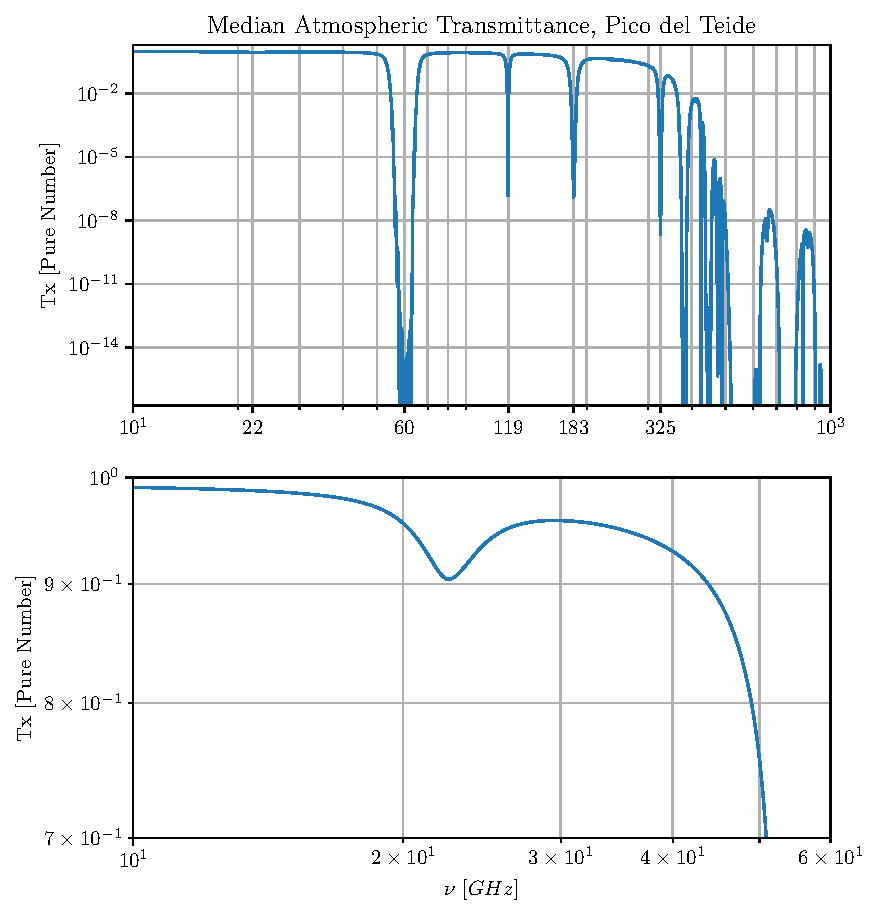
\includegraphics[width=\textwidth]{transmittance_Teide}
        \caption{Atmospheric transmittance at Pico del Teide and low
        frequencies detail. CAL software.}
        \label{fig:transmittance_teide}
\end{figure}


The real and imaginary parts of $\epsilon$ are related to the atmopshere
refractive index, $n\qty(\nu)$, and absorption coefficient, $\alpha\qty(\nu)$,

\begin{align}
        \epsilon_r\qty(\nu) & = \sqrt{n\qty(\nu)} \\
        \epsilon_i\qty(\nu) & = \frac{\lambda \alpha\qty(\nu)}{4\pi}
\end{align}

where $\lambda$ is the wavelength of the incoming radiation.

From \autoref{eq:kk_relations_1} and \autoref{eq:kk_relations_2} follows that
the refractive index and the absorption coefficient are note independent
quantities.

\subsection{Essential Quantities in Radiative Transfer Theory}

When the scale of a system greatly exceed the wavelength of propagating
radiation, we can consider radiation to travel in straight line, called
\emph{rays} \autocite{rybicki2008radiative}. Starting from this observation
we can devise a theory of propagating rays, knwon as the \emph{radiative
transfer theory}.

We consider an infinitesimal area $\dd{A}$ normal to the direction of a
specific ray and we take into account all the rays passing through $\dd{A}$
whose direction is whithin an infinitesimal solid angle $\dd{\Omega}$ of
the given ray (see \autoref{fig:rays_geometry}). The energy crossing
$\dd{A}$ in an infinitesimal time $\dd{t}$, in a frequency range $\dd{\nu}$
is

\begin{equation}
        \dd{E} \equiv
        I\qty(\vb{x},\Omega,\nu)\dd{A}dd{\Omega}\dd{\nu}\dd{t}
\end{equation}

which defines the \emph{specififc intensity}, $I\qty(\vb{x},\Omega,\nu) =
I_\nu$.

\begin{figure}
        \centering
        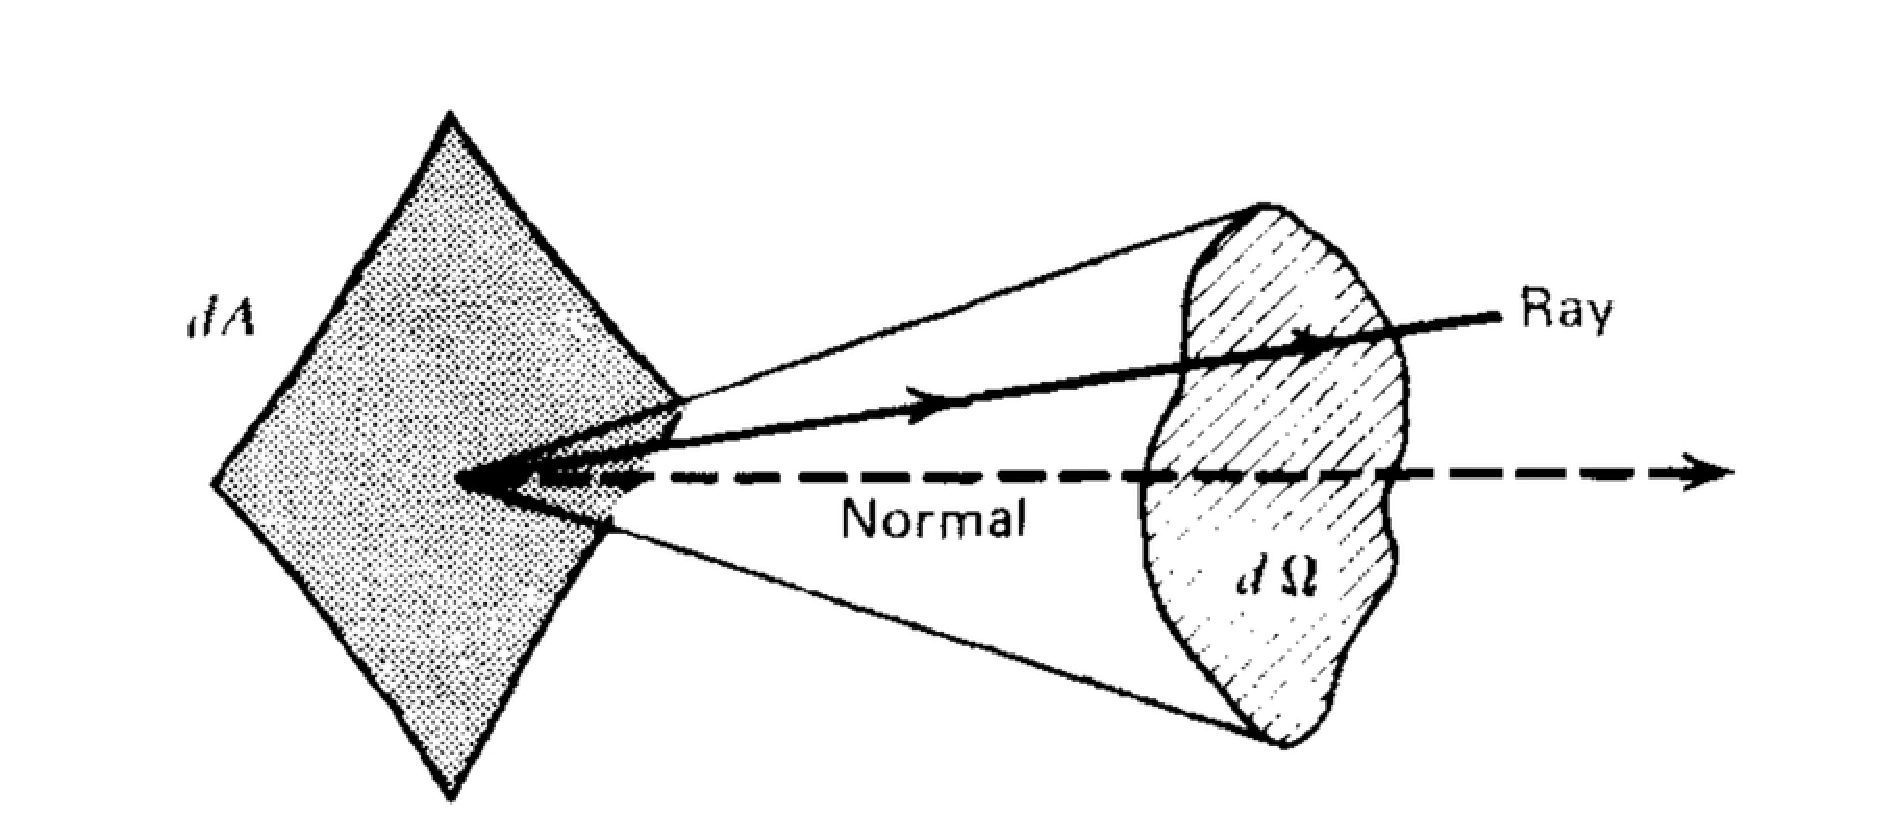
\includegraphics[width=\textwidth]{rays_geometry}
        \caption{Geometry for normally incident rays
        \autocite{rybicki2008radiative}.}
        \label{fig:rays_geometry}
\end{figure}

The absorption coefficient $\alpha\qty(\nu) = \alpha_\nu$, introduced in the
previus section, represents the loss of intensity in a beam as it travels an
infinitesimal distance $\dd{r}$ in a dispersive medium. As the radiation
proceeds in the material, it runs into a random distribution of absorbers,
each presenting a cross section $\sigma_\nu$, of number density $n$. If we
assume that the mean interparticle distance is large in comparison to the
linear scale of the cross section, that is $n^{-\frac{1}{3}} \gg
\sqrt{\sigma_\nu}$, the total energy absorbed out of a beam passing
through a infinitesimal area $\dd{A}$ within a solid angle $\dd{\Omega}$ is

\begin{equation}
        \dd{E} = I_\nu \sigma_\nu n \dd{V} \dd{\Omega} \dd{\nu} \dd{t}
\end{equation}

where $\sigma_\nu n \dd{V} = \sigma_\nu n \dd{A} \dd{r}$ is the total
absorbing area presented by absorbers. The loss in energy, by definition,
can be expressed in terms of specifc brightness:

\begin{equation}
        \dd{E} = -\dd{I_\nu} \dd{A} \dd{\Omega} \dd{\nu} \dd{t}.
\end{equation}

Therefore if we combine the last two equations, we obtain

\begin{equation}
        \dv{I_\nu}{r} = -\sigma_\nu n I_\nu
        \label{eq:absorption}
\end{equation}

where $\sigma_\nu n = \alpha_\nu$. Note that absorption in
\autoref{eq:absorption} includes both \emph{true absorption} and
\emph{stimulated emission}, because both are proportional to the intensity
of the incoming radiation. Thus, $\alpha$ can be a positive or a negative
quantity.

The spontaneous emission, on the other hand, is independent of the
specific intensity of the beam. In the contest of radiative transfer theory
the quantity linked to this phenomenon is the \emph{spontaneous emission
coefficient} $j$, which is defined as the energy emitted
per unit time per unit solid angle and per unit volume:

\begin{equation}
        \dd{E} \equiv j\dd{V}\dd{\Omega}\dd{t}.
\end{equation}

A \emph{monochromatic spontaneous emission coefficient}, $j\qty(\nu) =
j_\nu$, can also be defined as

\begin{equation}
        j \equiv j_\nu \dd{\nu}.
\end{equation}

From now on we will refer to this quantity simply as the \emph{emission
coefficient}.
A beam of cross section $\dd{A}$, travelling an infinitesimal distance
$\dd{r}$, goes through a volume $\dd{V} = \dd{A} \dd{r}$. Therefore, from
the last two equations, we have

\begin{equation}
        \begin{split}
        \frac{\dd{E}}{\dd{A}\dd{\Omega}\dd{\nu}\dd{t}} & = j_\nu \dd{r} \\
        \dv{I_\nu}{r} & = j_\nu
        \label{eq:emission}
        \end{split}
\end{equation}

\subsection{The Radiative Transfer Equation}\label{ss:radiative_transfer_eq}

The effects of emission and absorption can be incorporated into a sigle
equation giving the variation of specific intensity. From \autoref{eq:absorption}
and \autoref{eq:emission} we have

\begin{equation}
        \dv{I_\nu}{r} = -\alpha_\nu I_\nu + j_\nu
\end{equation}

which is known as the \emph{radiative transfer equation}. This equation
takes a particularly simple for if we realize the change of variable

\begin{equation}
        \begin{split}
                r \rightarrow \tau_\nu\qty(r) & \equiv \int^r_{r_0}
                \dd{r'}\alpha_\nu\qty(r') \\
                \dd{\tau_\nu} & = \alpha_\nu \dd{r}
        \end{split}
\end{equation}

where $\tau_\nu$ is known as the \emph{optical depth} or \emph{opacity}
\autocite{rybicki2008radiative}.
The transfer equation can now be divided by $\alpha_\nu$ and written as

\begin{equation}
        \dv{I_\nu\qty(\tau_\nu)}{\tau_\nu} = -I_\nu(\tau_\nu) +
        S_\nu\qty(\tau_\nu)
        \label{eq:radiative_transfer}
\end{equation}

where the function $S_\nu\qty(\tau_\nu)$ is known as the as the \emph{source
function} and is defined as

\begin{equation}
        S_\nu(\tau_\nu) \equiv
        \frac{j_\nu\qty(\tau_\nu)}{\alpha_\nu\qty(\tau_\nu)}.
\end{equation}

The source function and the opacity are convenient quantities in radiative
transfer theory, because they allow to reveal more clearly the intervals
along a ray that influence propagation of radiation the most.

\autoref{eq:radiative_transfer} can be now solved by regarding all
quantities as a function of the optical depth. First we multiply each side
of the equation by the positive quantity $e^{\tau_\nu}$:

\begin{equation}
        \dv{I_\nu\qty(\tau_\nu)}{\tau_\nu}e^{\tau_\nu} =
        -I_\nu\qty(\tau_\nu)e^{\tau_\nu} +
        S_\nu\qty(\tau_\nu)e^{\tau_\nu}
\end{equation}

then we integrate along a vertical path through the atmosphere:

\begin{equation}
        \begin{split}
                & \int^{\tau_{A,\nu}}_0 \dd{\tau_\nu}
                \dv{I_\nu\qty(\tau_\nu)}{\tau_\nu} e^{\tau_\nu} =
                -\int^{\tau_{A,\nu}}_0 \dd{\tau_\nu}
                I_\nu\qty(\tau_\nu) e^{\tau_\nu} +
                \int^{\tau_{A,\nu}}_0 \dd{\tau_\nu}
                S_\nu\qty(\tau_\nu) e^{\tau_\nu} \\
                & \eval{I_\nu\qty(\tau_\nu) e^\tau}^{\tau_{A,\nu}}_0
                -\int^{\tau_{A,\nu}}_0 \dd{\tau_\nu}
                I_\nu\qty(\tau_\nu) e^{\tau_\nu} = \\
                & = -\int^{\tau_{A,\nu}}_0 \dd{\tau_\nu}
                I_\nu\qty(\tau_\nu) e^{\tau_\nu} +
                \int^{\tau_{A,\nu}}_0 \dd{\tau_\nu}
                S_\nu\qty(\tau_\nu) e^{\tau_\nu} \\
                & I_\nu\qty(\tau_{A,\nu}) e^{\tau_{A,\nu}} -I_\nu\qty(0) =
                \int^{\tau_{A,\nu}}_0 \dd{\tau_\nu}
                S_\nu\qty(\tau_\nu) e^{\tau_\nu}
        \end{split}
\end{equation}

where integration by parts has been used in the right-hand side of the
equation and the quantity $\tau_{A,\nu}$ is the total opacity of the
traversed medium. If the last equation is divided by the positive factor
$e^{\tau_{A,\nu}}$ and terms are remanaged, the following equation is
obtained:

\begin{equation}
        I_\nu\qty(\tau_{A,\nu}) = I_\nu\qty(0) e^{-\tau_{A,\nu}} +
        \int^{\tau_{A,\nu}}_0 \dd{\tau_\nu}
        S_\nu\qty(\tau_\nu) e^{-\qty(\tau_{A,\nu} - \tau_\nu)}.
\end{equation}

This is known as the \emph{formal solution} of the radiative transfer
equation. The term $I_\nu\qty(0) e^{-\tau_{A,\nu}}$ represents the initial
intensity diminished by absorption and the second term in the sum stands
for the integrated source diminished by absorption.

\subsection{A Solution for Thermal Sources}

Thermal radiation is radiation emitted by matter in thermodynamic
equilibrium. When radiation is itself in thermodynamic equilibrium we
speak about \emph{black body radiation}, whose nature was already described
in \autoref{ss:cmb_bb}.

For black body radiation we have

\begin{equation}
        I_\nu \equiv B_\nu\qty(T_\text{phys})
\end{equation}

where $T_\text{phys}$ is the physical temperature of the radiation and of the
emitter and $B_\nu\qty(T_\text{phys})$ is the black body spectrum introduced
in \autoref{ss:cmb_bb},

\begin{equation}
        B_\nu\qty(T) = \frac{2h\nu^3}{c^2}
        \frac{1}{\exp(\frac{h\nu}{K_b T}) - 1}.
\end{equation}

This means that for black body radiation $I_\nu$ is an universal function
of $T$ and $\nu$, independent of the properties of the emitting body.

Kirchhoff's law states that the source function of a body in thermodynamic
equilibrium coincides with a black body spectrum

\begin{align}
        S_\nu & = B_\nu\qty(T_\text{phys}) \\
        j_\nu & = B_\nu\qty(T_\text{phys}) \alpha_\nu
\end{align}

where $T_\text{phys}$ is the physical temperature of the radiant body,
which from now on will be referred to simply as T.

The solution of the radiative transfer equation in the case of thermal
radiation is obtained from the formal solution by substitution of the
correct source function:

\begin{equation}
        I_\nu\qty(\tau_{A,\nu}) = I_\nu\qty(0) e^{-\tau_{A,\nu}} +
        \int^{\tau_{A,\nu}}_0 \dd{\tau_\nu} B_\nu\qty(T\qty(\tau_\nu))
        e^{-\qty(\tau_{A,\nu} - \tau_\nu)}.
        \label{eq:radiative_thermal}
\end{equation}

A further approximation can be made to simplify this result.
The exponential term in the Planck law can be expanded as

\begin{equation}
       \exp(\frac{h\nu}{K_b T}) = 1 + \frac{h\nu}{K_b T} + \order{\nu^2}.
\end{equation}

Therefore, for $\frac{h \nu}{K_b T}$, we obtain the \emph{Rayleigh-Jeans
approximation law} (see for example \cite{condon2016essential}):

\begin{equation}
        B_\nu\qty(T) \approx \frac{2\nu^2}{c^2} K_b T.
\end{equation}

This relation is commonly used in astrophysics to characterize the
brightness of a radiation at a certain frequency. For any value value of
$I_\nu$ a corresponding \emph{brightness temperature} temperature can be
defined as

\begin{equation}
        I_\nu \equiv B_\nu\qty(T_b)
\end{equation}

or assuming that the Rayleigh-Jeans approximation is valid,

\begin{equation}
        T_b \equiv = \frac{c^2}{2\nu^2k} I_\nu.
\end{equation}

So, \autoref{eq:radiative_thermal} can be rewritten as

\begin{equation}
        T_b = T_b\qty(0) e^{-\tau_{A,\nu}} +
        \int^{\tau_{A,\nu}}_0 \dd{\tau_\nu} T\qty(\tau_\nu)
        e^{-\qty(\tau_{A,\nu} - \tau_\nu)}.
\end{equation}

The solution of this equation in the case of constant temperature along the
optical path, $T\qty(\tau_\nu) = T = \text{const.}$ is

\begin{equation}
        T_b = T_b\qty(0) e^{-\tau_{A,\nu}} + T\qty(1 -
        e^{-\tau_{A,\nu}}).
        \label{eq:rte_solution_thermal}
\end{equation}

If the opacity is large, the brightness temperature of the radiation
approaches the temperature of the medium.

\subsection{Local Thermodynamic Equilibrium}

It is possible to rewrite the radiative transfer equation in terms of
microscopic quantities. The theorical framework for the simple case of a
medium composed of emitters and absorbers characterized by two energy
levels was established by Einstein \autocite{einstein1917the},
in his famous article about the quantum theory of radiation.
The transfer equation in terms of Einstein coefficients reads

\begin{equation}
        \dv{I_\nu}{r} = -\frac{h\nu}{4\pi}\qty(n_1 B_{12} -
        n_2 B_{21})\phi\qty(\nu)I_\nu +
        \frac{h\nu}{4\pi} n_2 A_{21}\phi\qty(\nu)
\end{equation}

where

\begin{itemize}
        \item $n_1$ and $n_2$ are the number densities of atoms in energy
        levels 1 and 2, with $E_2 = E_1 + h\nu_0$;
        \item $B_{12}$ and $B_{21}$ are the Einstein absorption and
        stimulated emission coefficients, respectively;
        \item $A_{21}$ is the Einstein stimulated emission coefficient;
        \item and $\phi\qty(\nu)$ is the \emph{line profile function},
        which accounts for the fact that the energy difference $h\nu_0$i
        is not infinitely sharp. The line profile function is peaked at
        $\nu = \nu_0$ and is taken to be normalized:

        \begin{equation}
                \int^\infty_0 \phi\qty(\nu) = 1.
        \end{equation}

\end{itemize}

A comparison of this equation with \autoref{eq:radiative_transfer} allows
to obtain

\begin{align}
        \alpha_\nu & = \frac{h\nu}{4\pi}\qty(n_1 B_{12} -
        n_2 B_{21})\phi\qty(\nu) \\
        S_\nu & = \frac{n_2 A_{21}}{n_1 B_{12} - n_2 B_{21}}
\end{align}

which are the expressions for the absorption coefficient and the source
fuction in terms of microscopic quantities.

Using the Einstein \emph{detailed balance relations} for absorption and
emission (see for example \cite{rybicki2008radiative})

\begin{align}
        g_1 B_{12} & = g_2 B_{21} \\
        A_{21} & = \frac{2h\nu^3}{c^2} B_{21}
\end{align}

where $g_1$ and $g_2$ are statistical weights for energy level 1 and 2,
respectively, the absorption coefficient and the source function can be
rewritten as

\begin{align}
        \alpha_\nu & = \frac{h\nu}{4\pi} n_1 B_{12}
        \qty(1 - \frac{g_1 n_2}{g_2 n_1})\phi\qty(\nu)\\
        S_\nu & = \frac{2h\nu^3}{c^2}\qty(\frac{g_2 n_1}{g_1 n_2} - 1)^{-1}.
        \label{eq:gen_kirchhoff_law}
\end{align}

\autoref{eq:gen_kirchhoff_law} is known as the \emph{generalized Kirchhoff
law} and is valid even out of thermodinamic equilibrium. For a thermalized
system the number density for a certain energy level $i$, $n_i$, is
proportional to the \emph{Boltzmann dustribution} and to its degeneracy
number, $g_i$,

\begin{equation}
        n_i \propto \frac{g_i}{Q} \exp(-\frac{E_i}{K_b T})
\end{equation}

where

\begin{equation}
        Q \equiv \sum_j \exp(-\frac{E_j}{K_b T})
\end{equation}

is the \emph{canonical partition function}. The j index in the sum runs
over all states that are accessible to the to system. Therefore, in the
case of our two levels system we have that

\begin{equation}
        \frac{n_1}{n_2} = \frac{g_1 \exp(-\frac{E}{K_b T})}{
        g_2 \exp(-\frac{E + h\nu_0}{K_b T})} =
        \frac{g_1}{g_2} \exp(\frac{h\nu_0}{K_b T})
\end{equation}

and the expression for the absorption coefficient and the source function
become

\begin{align}
        \alpha_\nu & = \frac{h\nu}{4\pi} n_1 B_{12}
        \qty[1 - \exp(-\frac{h\nu}{K_b T})]\phi\qty(\nu)\\
        S_\nu & = \frac{2h\nu^3}{c^2}\qty[\exp(\frac{h\nu}{K_b T}) - 1]^{-1}
        = B_\nu\qty(T).
\end{align}

This thermal value for the source function is just a statement of the
Kirchhoff law. In this case matter is in thermal equilibrium with
itself but not necessarily with radiation, so it is said to be in \emph{local
thermodynamic equilibrium} (LTE). The atmosphere is in fact a dispersive
medium in local thermodinamic equilibrium: cosmic electromagnetic waves
such as solar radiation, the CMB, and radiations from the galaxy propagate
through it, but they are not in thermodinamic equilibrium with the medium.

Of course our atmosphere is not an ensamble of two levels emitters and
absorbers, like the one we have presented above. Instead, it is in local
thermodinamic equilibrium in a classical sense: the local distribution of
particle velocities within it corresponds to the \emph{Maxwell-Boltzmann}
distribution,

\begin{equation}
        p\qty(v) = \qty(\frac{m_*}{2\pi K_b T})^{3/2}
        \exp(-\frac{m_* v^2}{2 K_b T})
\end{equation}

where $m_*$ is a reference mass for particles in the atmosphere.
This means that in principle we can split the atmosphere in an arbitrary
number of vertical layers, assuming the thermodynamic temperature is
constant within each one.  The radiative transfer equation can then be
written down and solved for every layer and the solutions connected. This
constitutes a simplified view of the numerical approach we have adopted in
the context of this thesis to obtain estimates for atmospheric brightness
temperatures.

\section{Atmospheric Spatial Structures}

As already mentioned in \autoref{ss:atmosphere_problem}, water
vapour is found in the atmosphere in highly variable concentrations and so
it has a great influence on fluctuations in the values of the refractive
index, $n_\nu$, and the absorption coefficient, $\alpha_\nu$. For frequncies
below \SI{100}{\giga\hertz}, simple empirical expressions for those
contribution are available. The refractivity, $N_\nu$, is defined as

\begin{equation}
        N_\nu = \num{e6}\qty(n_\nu - 1)
\end{equation}

and in this wavelength range is approximately a constant function of
frequency, $N\qty(\nu) = N$, given by the Smith-Weintraub equation
\autocite{smith1953constants}:

\begin{equation}
        N = 77\frac{P_d}{T} + 64.8\frac{P_v}{T} +
        \num{3.776e5}\frac{P_v}{T^2}.
\end{equation}

Here $P_d$ is the partial vapour pressure of dry air in
\si{\milli\bar}, $P_v$ is the partial wapter vapour pressure in the same
unit measure and T is the physical atmosphere temperature in \si{\kelvin}.
Fluctuations in the value of the refractive index as the air drift through
the instrument beam cause variations in the path length from a source to
the telescope. For CMB radiation experiments with beamsizes of a degree or
more that observe at \si{\centi\meter} wavelengths, these effects are small
and can be ignored \autocite{church1995predicting}.

The low frequnecy contribution to $\alpha_\nu$ is governed by the
\SI{22}{\giga\hertz} water vapour transition (see
\autoref{fig:transmittance_teide}) and is given by that following simple
expression, which also includes a corrective terms for wings of other
lines \autocite{waters19762}:

\begin{equation}
        \alpha_\nu = \rho_v\nu^2\Delta \nu T^{-\frac{3}{2}}
        \qty[\frac{7.18}{T} e^{-\frac{644}{T}}
        \frac{1}{\qty(494.40190 - \nu^2)^2 + 4\nu^2\Delta \nu^2}
        + \num{2.77e-8}]
\end{equation}

where

\begin{equation}
        \Delta \nu = 2.96\qty(\frac{P}{1013})\qty(\frac{300}{T})^{0.626}
        \qty(1 + 0.018\frac{\rho_v T}{P})
\end{equation}

and $\rho_v$ is the water vapour density in \si{\gram\per\cubic\meter}, P
is the air pressure expressed \si{\milli\bar}, T is the atmospheric physical
temperature.

\subsection{Absorption Coefficient Fluctuations}

Radiative transfer theory allows us to estimate the fluctuations
in the antenna temperature measured by a certain instrument, which in turn
are caused by fluctuations in the absorption coefficient, $\alpha_\nu$.
\autoref{eq:radiative_thermal} can be rewritten in terms of the path length
travelled in the dispersive medium, reverting the change of variable $r
\rightarrow \tau_\nu$:

\begin{equation}
        T_\text{atm} = T_b - T_b\qty(0) e^{-\tau_{A,\nu}} =
        \int^R_0 \dd{r} \alpha_\nu\qty(r) T\qty(r) e^{-\tau_\nu}
        \label{eq:radiative_atm}
\end{equation}

where $T_\text{atm}$ is the atmospheric brightness temperature, which is
obtained subtracting from the total brighness temperature, $T_b =
T_\text{sky}$, the contribution from the cosmic radiations diminished by
the atmospheric absorption. If the effects of the clouds are ignored,
assuming that only clear sky observations will be used for CMB radiation
observation, the total atmopsheric opacity is small for low frequencies:
$\tau_{A,\nu} \sim \num{e-2}$. Consequently, fluctuations in atmospheric
brightness temperature arising from variations in $\tau_\nu$ constitute a
second order effect, when compared to fluctuations in the absorption
coefficient. Therefore, from now on, we assume that $e^{-\tau_\nu} \simeq
1$.

The \emph{effective area}, $A_\text{eff}$, of an instrument is defined as

\begin{equation}
        A_\text{eff}\qty(\nu) = \frac{P\qty(\nu)}{F\qty(\nu)}
\end{equation}

where $P_\qty(\nu)$ is the power per unit frequency measured by the
antenna and $S\qty(\nu)$ is the power per unit area and unit frequency emitted
from the source.
From \autoref{eq:radiative_atm} we deduce that the contribution to the
antenna temperature measured by an istrument of effective area
$A_\text{eff}$, pointing in the direction of the unit vector $\vectorunit{r}_s$ from an infinitesimal
element of path length $\dd{r}$ through the atmosphere at the position $\vb{r}$ is

\begin{equation}
        \dd{T_\text{A}} = \frac{1}{\lambda^2} A_{\text{eff},\nu}
        \qty(\vectorunit{r}_s,\vb{r}) \alpha_\nu\qty(\vb{r}) T\qty(\vb{r})
        \dd{\Omega}\dd{r}.
\end{equation}

If we integrate over all the volume of atmosphere we obtain:

\begin{equation}
        T_\text{A} = \frac{1}{\lambda^2} \int_V \frac{\dd{V}}{r^2}
        A_{\text{eff},\nu} \qty(\vectorunit{r}_s,\vb{r})
        \alpha_\nu\qty(\vb{r}) T\qty(\vb{r}).
\end{equation}

We assume now that the instrument is pointing at the
zenith. An instrument not pointing at the zenith will be looking through a
larger airmass and so the size of fluctuations will be increased.
The airmass $m\qty(\theta_\text{zth})$ ranges from \num{1} at the zenith to
about \num{40} at the horizon and can be computed for any zenith angle
using the following empirical formula \autocite{errard2015modeling}:

\begin{equation}
        m\qty(\theta_\text{zth}) \propto
        \frac{1}{\cos \theta_\text{zth} + 0.50572
        \qty(96.07995 - \theta_\text{zth}[\text{deg}])^{-1.6364}}.
\end{equation}

A change of variables to cartesian coordinates results in the following
expression for the antenna temperature:

\begin{equation}
        T_\text{A} = \frac{1}{\lambda^2} \int^{z_u}_0 \int^{x_2}_{x_1}
        \int^{y_2}_{y_1} \frac{\dd{x}\dd{y}\dd{z}}{x^2 + y^2 + z^2}
        A_{\text{eff},\nu}\qty(x,y,z)
        \alpha_\nu\qty(x,y,z) T\qty(x,y,z)
\end{equation}

where we are performing the integration over a volume delimited by the
points $x_1$, $x_2$, $y_1$, $y_2$, 0, $z_u$. $z = 0$ corresponds to
the ground; $z_u$ is the height of the atmosphere; $x_i$ and $y_i$ set the
limits of the box in the horizontal directions. Beyond this coordinates the
contribute to the antenna temperature from an element of the atmosphere
become negligible.

If the beam is assumed to be narrow and the temperature to be a function
of the height only, $T\qty(x,y,z) \equiv T\qty(z)$, the last equation
becomes

\begin{equation}
        T_\text{A} = \frac{1}{\lambda^2} \int^{z_u}_{z_c}
        \iint^\infty_{-\infty} \frac{\dd{x}\dd{y}\dd{z}}{z^2}
        A_{\text{eff},\nu}\qty(x,y,z)
        \alpha_\nu\qty(x,y,z) T\qty(z)
        \label{eq:fluctuations_t_antenna}
\end{equation}

where $z_c$ is a cut off value which assures that the narrow beam
condition, $x,y \ll z$, is satisfied over the whole integration domain.
The gain drops rapidly for $z < z_c$ and the effect of imposing an
arbitrary cutoff is negligible.

The random mean squared fluctuations in antenna temperature due to variations in
the absorption coefficients are

\begin{equation}
        \begin{split}
                \expval{\var{T^2_\text{A}}} = & \frac{1}{\lambda^2}
                \int^{z_u}_{z_c}\iint^\infty_{-\infty}
                \int^{z_u}_{z_c}\iint^\infty_{-\infty}
                \frac{\dd{x_1}\dd{y_1}\dd{z_1}}{z^2_1}
                \frac{\dd{x_2}\dd{y_2}\dd{z_2}}{z^2_2} \times \\
                & \times A_{\text{eff},\nu}\qty(x_1,y_1,z_1)
                A_{\text{eff},\nu}\qty(x_2,y_2,z_2) \times \\
                & \times \expval{\var{\alpha_\nu}\qty(x_1,y_1,z_1)
                \var{\alpha_\nu}\qty(x_2,y_2,z_2)}
                T\qty(z_1)T\qty(z_1).
        \end{split}
        \label{eq:rms_t_antenna}
\end{equation}

Consequently the complexity in the calculation of atmospheric brightness
temperature fluctuations is transferred to the correlation function for
fluctuations in the absorption coefficient.

\subsection{The Turbulent Structure of the Atmosphere}\label{ss:turbulent_structure}

In literature the turbulent structure of the atmosphere is assumed to be
described by the \emph{Kolmogorov-Taylor model} in which the turbulence has
a Kolmogorov spatial spectrum and the spatial features remain fixed as the
atmosphere is drifted through the beam by wind. This assumption is
known as the \emph{Taylor approximation} and excludes any effects of
variation of the speed of wind with height or any convective motions
\autocite{church1995predicting}.
The fluctuations in atmospheric brightness temperature are related to the
structure fuction of fluctuations in the absorption coefficient:

\begin{equation}
        \begin{split}
                \mathcal{D}_\alpha\qty(\vb{r}_1,\vb{r}_2) & =
                \expval{\qty[\alpha_\nu\qty(\vb{r}_1) -
                \alpha_\nu\qty(\vb{r}_2)]^2} =
                \\
                & = B_\alpha\qty(\vb{r}_1,\vb{r}_1) -
                2B_\alpha\qty(\vb{r}_1,\vb{r}_2) + B_\alpha\qty(\vb{r}_2,\vb{r}_2)
        \end{split}
\end{equation}

where

\begin{equation}
        B_\alpha\qty(\vb{r}_1,\vb{r}_2) =
        \expval{\alpha_\nu\qty(\vb{r}_1)\alpha_\nu\qty(\vb{r}_2)}.
\end{equation}

Assuming that turbolence is locally homogeneous and isotropic, the correlation
function $B_\alpha\qty(\vb{r}_1,\vb{r}_2)$ can be written as the product of
a squared amplitude, witch depends on the coordinates, and a function that
depends only on the separation between the two points of interest
\autocite{tatarski2016wave}:

\begin{equation}
        B_\alpha\qty(\vb{r}_1,\vb{r}_2) = \frac{1}{2}
        C^2_\alpha\qty(\abs{\vb{r}_1 + \vb{r}_2})
        L^{\frac{2}{3}}_0 b_\alpha\qty(\abs{\vb{r}_1 - \vb{r}_2}),\quad
        l_0 \ll \abs{\vb{r}_1 - \vb{r}_2} \ll L_0
\end{equation}

where $b_\alpha\qty(\abs{\vb{r}_1 - \vb{r}_2})$ is the normalized version
of the correlation function and

\begin{equation}
        b_\alpha\qty(\abs{\vb{r}_1 - \vb{r}_2}) \propto
        \abs{\vb{r}_1 - \vb{r}_2}^\frac{2}{3}.
\end{equation}

The parameters $l_0$ and $L_0$ are typical the inner and outer distance
scales of the atmospheric structures over which the $2/3$ law holds.
Measurements of $L_0$ fluctuations in the optical and radio regime shows
that $L_0 \sim \SI{e1}{\meter}$. However, large uncertainties in the value
of the outer scale must be expected, this parameter strongly
depends on weather conditions.

The normalized Kolmogorov correlation function, $b_\alpha\qty(\abs{\vb{r}_1 - \vb{r}_2})$ can be related to a
spherically symmetric power spectrum $\phi\qty(k)$:

\begin{equation}
        b_\alpha\qty(\Delta r) \propto \frac{1}{\Delta r}
        \int^{k_\text{max}}_{k_0} \dd{k} k \phi\qty(k) \sin(k\Delta r)
\end{equation}

where $\phi\qty(k) \propto k^{11/3}$ represents the Kolmogorov model, $k_0
\sim 1/L_0$, $k_\text{max} \sim 1/l_0$ and $\Delta r = \abs{\vb{r}_1 -
\vb{r}_2}$ \autocite{tatarski2016wave}. \autoref{fig:kt_spectrum} shows the
depence of the Kolmogorov normalized correlation function on the outer
scale $L_0$.

\begin{figure}
        \centering
        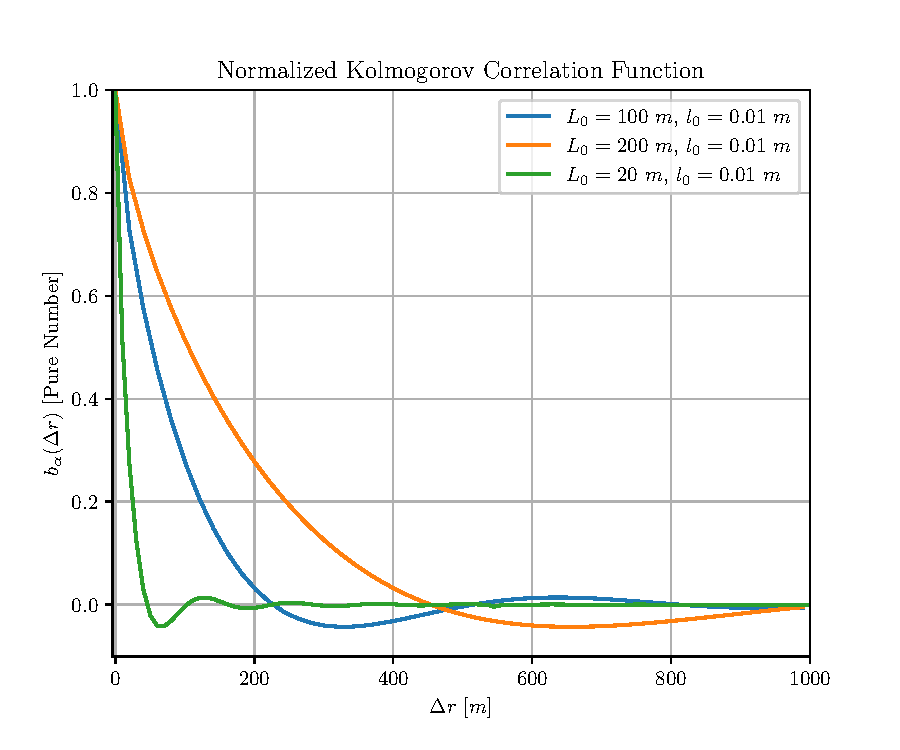
\includegraphics[width=\textwidth]{kt_spectrum}
        \caption{Normalized Kolmogorov correlation function.}
        \label{fig:kt_spectrum}
\end{figure}

In the radio regime, the squared amplitude appearing in the absorption
coefficient correlation function is related to the atmospheric water vapour
content by

\begin{equation}
        C^2_\alpha = a L^\frac{4}{3}_0 \qty(\fdv{\alpha_\nu}{q}
        \dv{q}{z})^2
\end{equation}

where $a$ is a positive constant and $q = \rho_v/1.62p$ is the specific umidity
\autocite{tatarski2016wave}.  Thus, the height dependence of $C^2_\alpha$
is strongly influenced by the height distribution of water vapour. This
dependence is difficult to model and here we follow Church assuming a
simple model: $C^2_\alpha \propto \rho_v$. The height
dependence of water vapour density is assumed to be approximated by an
exeponential distribution:

\begin{equation}
        \rho_v\qty(z) = \rho_{v,0} \exp(-\frac{z}{z_0})
\end{equation}

where $\rho_{v,0}$ is the ground water vapour density and $z_0$ is a scale
height for the exponential decay. Therefore, the amplitude function for the
absorption coefficient correlation function is

\begin{equation}
        C^2_\alpha = C^2_0\exp(-\frac{z}{z_0}).
\end{equation}

\subsection{Random Fluctuations in Antenna Temperature}

Random fluctuations in antenna temperature, caused by fluctuations in the
absorption coefficient, can now be estimed for a specific instrument using
\autoref{eq:rms_t_antenna}. We consider the simple case of a single dish
system, making the further assumption that the beam patter as a function of
height can be described by the propagation of a single Gaussian mode.
In this case the electronic field propagating in the $z$-direction is the
simplest eigenfunction of the \emph{Huygens integral operator}
\autocite{belanger1991beam}

\begin{equation}
        \begin{split}
                \mathcal{H}\qty[E\qty(x_1,y_1,z_1)] = &
                \frac{i}{\lambda \qty(z - z_1)} e^{-ik\qty(z - z_1)} \times \\
                & \times \iint \dd{x_1}\dd{y_1} E\qty(x_1,y_1,z_1)
                e^{-ik\qty[\frac{\qty(x - x_1)^2 +
                \qty(y - y_1) ^2}{2\qty(z - z_1)}]}
        \end{split}
\end{equation}

which is known as the gaussian \emph{Laguerre-Gauss mode}
\autocite{alda2003laser}:

\begin{equation}
        E\qty(x,y,z) = E_0 \frac{w_0}{w\qty(z)} e^{-ikz + i\zeta\qty(z)}
        e^{-\frac{r^2}{w^2\qty(z)}} e^{-i\frac{kr^2}{2R\qty(z)}}
\end{equation}

where

\begin{align}
        w\qty(z) & = w_0 \sqrt{1 + \qty(\frac{z}{z_R})^2} \\
        R\qty(z) & = \frac{z^2_R}{z}\qty[1 + \qty(\frac{z}{z_R})^2] \\
        \zeta\qty(z) & = \arctan(\frac{z}{z_R}).
\end{align}

The function $\zeta\qty(z)$ is a phase factor known as the \emph{Guoy phase
shift}; $z_R = \pi w_0^2/\lambda$ is the \emph{Rayleigh range} and $w_0$ is
the \emph{beam waist radius}, which is related to the full width half
maximum of the beam by

\begin{equation}
        \text{FWHM}\qty(z) = \sqrt{2\ln 2} w\qty(z) \simeq 1.177 w\qty(z).
\end{equation}

It can be shown that in this case the effective area of a dish pointing in
the $z$-direction is \autocite{church1995predicting}

\begin{equation}
        A_{\text{eff},\nu} = \frac{2\lambda^2 z^2}{\pi w^2\qty(z)}
        e^{-\frac{2 \qty(x^2 + y^2)}{w^2\qty(z)}}.
\end{equation}

Therefore, using \autoref{eq:rms_t_antenna}, the mean squared fluctuations
in antenna temperature are

\begin{equation}
        \begin{split}
                \expval{\var{T^2_\text{A}}} = & \frac{2 L^\frac{2}{3}_0}{\pi^2}
                \iint^\infty_{-\infty} \int^{z_u}_{z_c}
                \iint^\infty_{-\infty} \int^{z_u}_{z_c}
                \dd{x_1}\dd{y_1}\dd{z_1}\dd{x_2}\dd{y_2}\dd{z_2} \times \\
                & C^2_\alpha\qty(\frac{z_1 + z_2}{2})
                b_\alpha\qty(x_1 - x_2, y_1 - y_2, z_1 - z_2)
                T\qty(z_1) T\qty(z_2) \times \\
                & \times \frac{1}{w^2\qty(z_1) w^2\qty(z_2)}
                e^{-\frac{2\qty(x^2_1 + y^2_1)}{w^2\qty(z_1)}}
                e^{-\frac{2\qty(x^2_2 + y^2_2)}{w^2\qty(z_2)}}.
        \end{split}
        \label{eq:rms_t_antenna_sdish}
\end{equation}

We now make a numer of assumption to successfully perform the integration.
First we assume that

\begin{equation}
        z_1 - z_2 \ll z_1 + z_2.
\end{equation}

This is valid for $z \gg L_0$ and means that $w^2\qty(z_1) \simeq
w^2\qty(z_2)$. Than we choose an approximated form for the normalized
Kolmogorov correlation function, which can be easily integrated.
\autoref{fig:kt-gaussian_comparison_2} shows that a Gaussian approximation,

\begin{equation}
        b_\alpha\qty(\Delta r) = e^{-\frac{\Delta r^2}{2L^2}},
        \qquad L = \frac{L_0}{4}
\end{equation}

is an appropriate choice. In particular this function understimates the
correlation on small scales and overestimates it on larger scales when
compared to the kolmogorov normalized correlation function.

\autoref{eq:rms_t_antenna_sdish} can now be easily integrated performing
convenient changes of variables. The result is

\begin{equation}
        \expval{\var{T^2_A}} = \sqrt{\frac{\pi}{32}} L^\frac{5}{3}_0
        \int^{z_u}_{z_c} \dd{Z} C^2_\alpha\qty(Z) T^2\qty(Z)
        \qty(1 + \frac{w^2\qty(Z)}{2L^2})^{-1}
\end{equation}

where $Z = \qty(z_1 + z_2)/2$i \autocite{church1995predicting}.

\begin{figure}
        \centering
        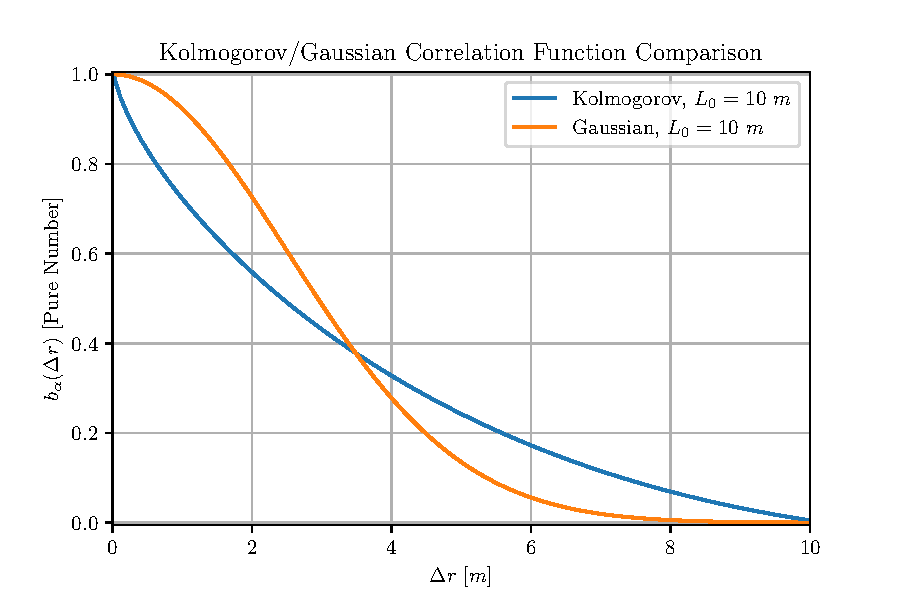
\includegraphics[width=\textwidth]{kt-gaussian_comparison_2}
        \caption{Kolmogorov/Gaussian normalized correlation fucntion
        comparison.}
        \label{fig:kt-gaussian_comparison_2}
\end{figure}

\autoref{fig:rms_t_outher_scale} shows the dependence of the fluctuations
in antenna temperature on the outher scale factor, $L_0$, assuming a sea
level temperature $T_0 = \SI{293}{\kelvin}$, with a linear decrease of $T\qty(z)
= T_0 - \SI{6.5e3}{\kelvin\per\meter}z$ to a maximum height of
\SI{2e3}{\meter} and beamsize of
\ang{;30;}. The parameters in the amplitude function are $C_{\alpha,0}
= \SI{2e-14}{\meter^{-8/3}}$ and $z_0 = \SI{2}{\kilo\meter}$. The fluctuations
in antenna temperature increase as the outher scale does, and
contributes to an extra amount of white noise load on detectors. For a
typical outher scale of \SI{e1}{\meter} the noise temperature is estimated
to be \SI{\sim e1}{\milli\kelvin}.

A significant reduction in the atmospheric
random fluctuations can be achieved deploying instruments
at dry, high altitudde sites, because of the amplitude factor $C^2_\alpha \propto
\exp(-z/z_0)$ appearing in the integral.

\begin{figure}
        \centering
        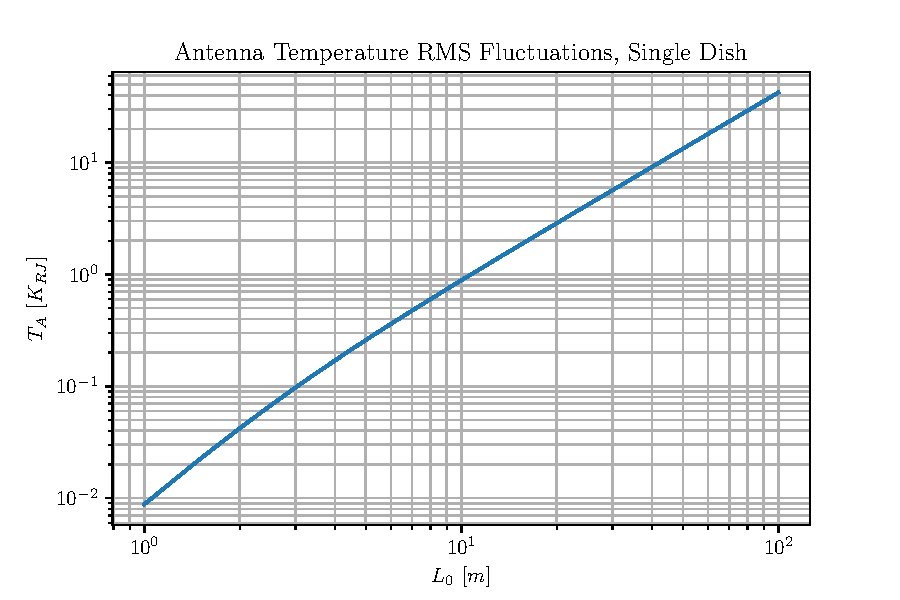
\includegraphics[width=\textwidth]{rms_t_outher_scale}
        \caption{Dependence of random fluctuations in antenna temperature
        on the outher scale of turbolence.}
        \label{fig:rms_t_outher_scale}
\end{figure}

\subsection{The Temporal Power Spectrum of Fluctuations in Antenna
Temperature}

To make realistic predictions of the effects of atmospheric emission, it is
now necessary to consider the temporal behaviour of the atmopsheric signal.
We derive here the temporal power spectrum for the same model system
presented in the previus subsection: a single dish instrument with beamsize
of \ang{;30;}, fixed and
pointing at the zenith.

The temporal power spectrum of atmospheric emission will depend on the
speed at which the atmosphere in dragged through the instrument beam by the
wind. It is convenient to select coordinate system coomoving with the
atmosphere. We choose the $x$-direction to be the wind direction. The
fluctuations in antenna temperature at a given time $t$ are obtained using
\autoref{eq:fluctuations_t_antenna}:

\begin{equation}
        \var{T_\text{A}} = \frac{1}{\lambda^2} \int^{z_u}_{z_c}
        \iint^\infty_{-\infty} \frac{\dd{x}\dd{y}\dd{z}}{z^2}
        A_{\text{eff},\nu}\qty(x - vt,y,z)
        \var{\alpha_\nu\qty(x,y,z) T\qty(z)}
\end{equation}

where $v$ is the wind speed in the $z$-direction. An expression for the
autocorrelation of the antenna temperature time fluctuations is derived
making use of the same assumptions and substitutions described in the
previous subsection:

\begin{equation}
        \begin{split}
                \expval{\var{T_A\qty(t)}\var{T_A\qty(t + t_*)}} = &
                \frac{L^{\frac{2}{3}}_0}{2\pi} \int^{z_u}_{z_c}
                \frac{\dd{Z}}{w^2\qty(Z)} C^2_\alpha\qty(Z)T^2\qty(Z) \times
                \\ \times
                & \iiint^\infty_{-\infty} b_\alpha\qty(\xi_x,\xi_y,\xi_z)
                \exp[-\frac{\qty(\xi_x + vt_*)^2 + \xi^2_y}{w^2\qty(Z)}]
        \end{split}
\end{equation}

where, in particular,

\begin{align}
         \xi_x & = x_1 - x_2 \\
         \xi_y & = y_1 - y_2 \\
         \xi_z & = z_1 - z_2 \\
         Z & = \frac{z_1 + z_2}{2}.
\end{align}

The power spectrum is obtained calculating the Fourier transform of the
latter expression:

\begin{equation}
        S\qty(\omega) = \frac{1}{\sqrt{2\pi}} \int^\infty_\infty \dd{t_*}
        e^{-i\omega t_*} \expval{\var{T_A\qty(t)}\var{T_A\qty(t + t_*)}}
\end{equation}

where $\omega$ is an angular frequency. In two important limiting cases,
corresponding to large and small outher scales, the Fourier transform of
the autocorrelation can be written as a product of two terms (see
\cite{church1995predicting}), $S\qty(\omega) =
I\qty(\omega/v)\Phi\qty(\omega/v)$. Where $I\qty(\omega/v)$ is the
instrumental filter on the temporal power spectrum, which is the same in
both of the cases, and $\Phi\qty(\omega,v)$ is the power spectrum itself.
In particular, if $b_\alpha\qty(\xi_x,\xi_y,\xi_z)$ is taken as the
Kolmogorov normalized correlation function,

\begin{itemize}
        \item If $w(Z) \gg L_0$:

        \begin{equation}
                \Phi\qty(\frac{\omega}{v}) \propto
                        \begin{cases}
                                \qty(\frac{\omega}{v})^{\frac{11}{3}} & \qif
                                \frac{1}{L_0} \ll \frac{\omega}{v}
                                \ll \frac{1}{l_0} \\
                                K & \qif \frac{\omega}{v} \ll \frac{1}{L_0}
                        \end{cases}
        \end{equation}

        \item If $w\qty(Z) \ll L_0$:

        \begin{equation}
                \Phi\qty(\frac{\omega}{v}) \propto
                        \begin{cases}
                                \qty(\frac{\omega}{v})^{\frac{8}{3}} & \qif
                                \frac{1}{L_0} \ll \frac{\omega}{v}
                                \ll \frac{1}{l_0} \\
                                K' & \qif \frac{\omega}{v} \ll \frac{1}{L_0}
                        \end{cases}
        \end{equation}
\end{itemize}

where $K$ and $K'$ are constants. The calculated power spectra for these
two limiting cases are showed in \autoref{fig:t_antenna_ps}. They were
obtained choosing $L_0 \sim \SI{1}{\meter}$ and $L_0 ~ \SI{100}{\meter}$,
respectively. In the real situation $L_0 \sim \SI{10}{\meter}$, so emission
at low altitude will contribute a spectrum with a $-8/3$ index and that at
high altitudes with a $-11/3$ index.

\begin{figure}
        \centering
        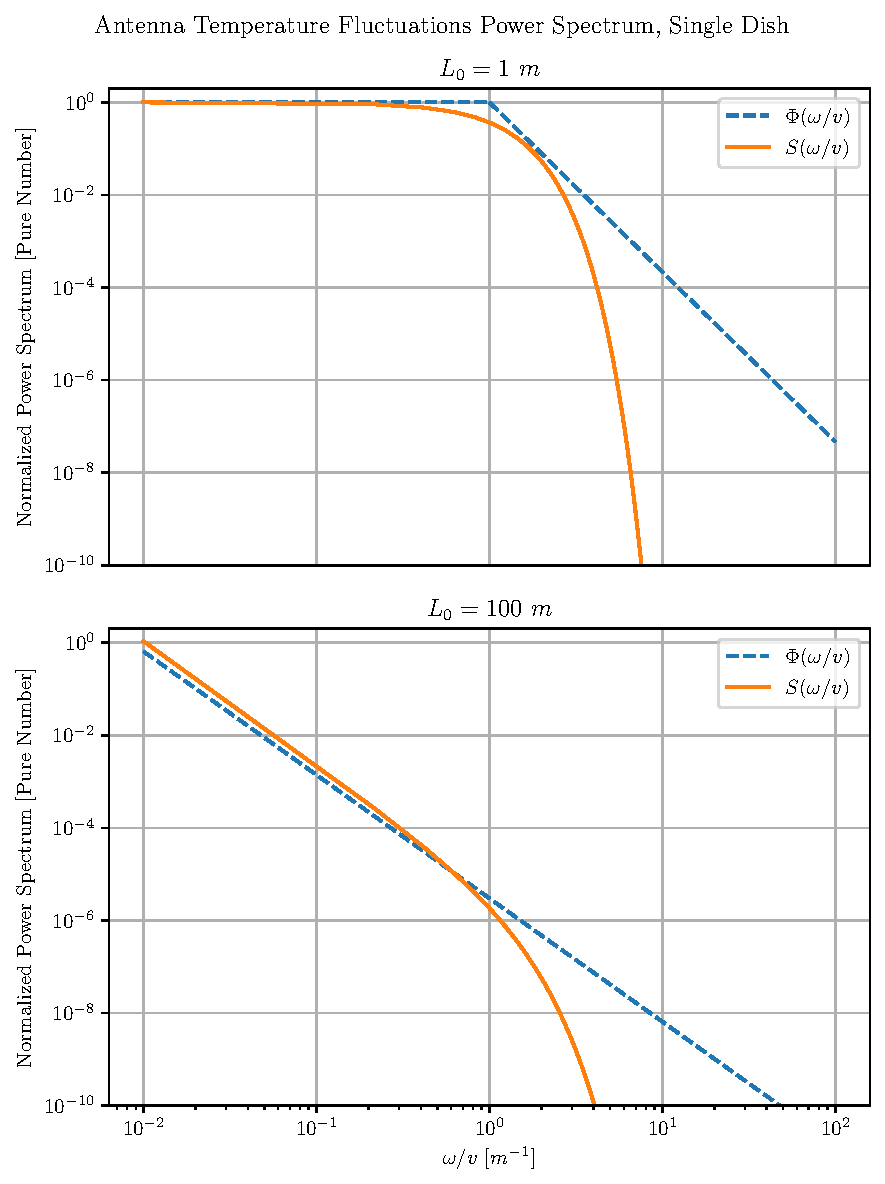
\includegraphics[width=\textwidth]{t_antenna_ps}
        \caption{Power spectra of the fluctautions in antenna temperature
        for a single dish system in the two limiting cases of large and
        small outher scale.}
        \label{fig:t_antenna_ps}
\end{figure}

\section{The Necessity of a Statistical Approch}

As has been shown in the current chapter, it's a complex task to model
the radiative contribution of our atmosphere. Atmospheric brighness
temperature in the microwave range depends on a set of
meteorological parameters, such as ground temperature; ground pressure;
total column liquid and iced water and wind speed. In addition,
white and correlated noise from atmospheric emission
srongly depends on total precipitable water vapour (PWV).
All of these quantities undergo seasonal and daily variations, thus
it is convenient to embrace a statistical approach.

The following chapters of these thesis will be devoted to realization of a
\emph{statistical picture} of the atmosphere at the site of the
Observatiorio del Teide and to the evaluation of the extra white noise
contribution on Strip detectors due to atmospheric effects. For the sake of
semplicity, atmospheric brighness temperature fluctuations, caused by
the turbulent structure of the atmosphere (see
\autoref{ss:turbulent_structure}), are not taken into account, but
are left to future works. Instead, the atmosphere will be treated as
uniform dispersive medium, bringing no correlation in time and
characterized by an absortion coefficient, $\alpha_\nu$, varying with
altitude.
